\documentclass{article}

\usepackage{fancyhdr}
\usepackage{extramarks}
\usepackage{amsmath}
\usepackage{amsthm}
\usepackage{amsfonts}
\usepackage{tikz}
\usepackage[plain]{algorithm}
\usepackage{algpseudocode}
\usepackage{listings} 
\usepackage{neuralnetwork}
\usetikzlibrary{automata,positioning}

\usepackage{color}

\definecolor{dkgreen}{rgb}{0,0.6,0}
\definecolor{gray}{rgb}{0.5,0.5,0.5}
\definecolor{mauve}{rgb}{0.58,0,0.82}

\lstset{frame=tb,
  language=Python,
  aboveskip=3mm,
  belowskip=3mm,
  showstringspaces=false,
  columns=flexible,
  basicstyle={\small\ttfamily},
  numbers=none,
  numberstyle=\tiny\color{gray},
  keywordstyle=\color{blue},
  commentstyle=\color{dkgreen},
  stringstyle=\color{mauve},
  breaklines=true,
  breakatwhitespace=true,
  tabsize=3
}
%
% Basic Document Settings
%

\topmargin=-0.45in
\evensidemargin=0in
\oddsidemargin=0in
\textwidth=6.5in
\textheight=9.0in
\headsep=0.25in

\linespread{1.1}

\pagestyle{fancy}
\lhead{\hmwkAuthorName}
\chead{\hmwkClass\: \hmwkTitle}
\rhead{\firstxmark}
\lfoot{\lastxmark}
\cfoot{\thepage}

\renewcommand\headrulewidth{0.4pt}
\renewcommand\footrulewidth{0.4pt}

\setlength\parindent{0pt}

%
% Create Problem Sections
%

\newcommand{\enterProblemHeader}[1]{
    \nobreak\extramarks{}{Task \arabic{#1} continued on next page\ldots}\nobreak{}
    \nobreak\extramarks{Task \arabic{#1} (continued)}{Problem \arabic{#1} continued on next page\ldots}\nobreak{}
}

\newcommand{\exitProblemHeader}[1]{
    \nobreak\extramarks{Task \arabic{#1} (continued)}{Problem \arabic{#1} continued on next page\ldots}\nobreak{}
    \stepcounter{#1}
    \nobreak\extramarks{Task \arabic{#1}}{}\nobreak{}
}

\setcounter{secnumdepth}{0}
\newcounter{partCounter}
\newcounter{homeworkProblemCounter}
\setcounter{homeworkProblemCounter}{1}
\nobreak\extramarks{Task \arabic{homeworkProblemCounter}}{}\nobreak{}

%
% Homework Problem Environment
%
% This environment takes an optional argument. When given, it will adjust the
% problem counter. This is useful for when the problems given for your
% assignment aren't sequential. See the last 3 problems of this template for an
% example.
%
\newenvironment{homeworkProblem}[1][-1]{
    \ifnum#1>0
        \setcounter{homeworkProblemCounter}{#1}
    \fi
    \section{Task \arabic{homeworkProblemCounter}}
    \setcounter{partCounter}{1}
    \enterProblemHeader{homeworkProblemCounter}
}{
    \exitProblemHeader{homeworkProblemCounter}
}

%
% Homework Details
%   - Title
%   - Due date
%   - Class
%   - Section/Time
%   - Instructor
%   - Author
%

\newcommand{\hmwkTitle}{Lab\ \#1}
\newcommand{\hmwkDueDate}{September 25, 2019}
\newcommand{\hmwkClass}{CSCI964 Computational Intelligence}
\newcommand{\hmwkClassTime}{2.14}
\newcommand{\hmwkClassInstructor}{Zhifeng Wang}
\newcommand{\hmwkAuthorName}{\textbf{Mei Wangzhihui}}
\newcommand{\hmwkAuthorNum}{\textbf{2019124044}}
%
% Title Page
%

\title{
    \vspace{2in}
    \textmd{\textbf{\hmwkClass:\ \hmwkTitle}}\\
    % \normalsize\vspace{0.1in}\small{Due\ on\ \hmwkDueDate\ at 3:10pm}\\
    % \vspace{0.1in}\large{\textit{\hmwkClassInstructor\ \hmwkClassTime}}
    \vspace{3in}
}

\author{\hmwkAuthorName\ \hmwkAuthorNum}
\date{}

\renewcommand{\part}[1]{\textbf{\large Part \Alph{partCounter}}\stepcounter{partCounter}\\}

%
% Various Helper Commands
%

% Useful for algorithms
\newcommand{\alg}[1]{\textsc{\bfseries \footnotesize #1}}

% For derivatives
\newcommand{\deriv}[1]{\frac{\mathrm{d}}{\mathrm{d}x} (#1)}

% For partial derivatives
\newcommand{\pderiv}[2]{\frac{\partial}{\partial #1} (#2)}

% Integral dx
\newcommand{\dx}{\mathrm{d}x}

% Alias for the Solution section header
\newcommand{\solution}{\textbf{\large Solution}}

% Probability commands: Expectation, Variance, Covariance, Bias
\newcommand{\E}{\mathrm{E}}
\newcommand{\Var}{\mathrm{Var}}
\newcommand{\Cov}{\mathrm{Cov}}
\newcommand{\Bias}{\mathrm{Bias}}

\begin{document}

\maketitle

\pagebreak

\begin{homeworkProblem}
\lstset{language=C}
\begin{lstlisting}
    #include <iostream>
    #include <eigen3/Eigen/Core>
    
    using namespace std;
    using namespace Eigen;
    
    double SigmoidFunc(double x)
    {
        return 1.0 / (1.0 + exp(-x));
    }
    
    void Sigmoid(VectorXf &src, VectorXf &dst)
    {
        float *src_data = src.data();
        float *dst_data = dst.data();
        for (int i = 0; i < src.size(); ++i)
        {
            dst_data[i] = SigmoidFunc(src_data[i]);
        }
    }
    
    double forwardProp(int numberOfLayers, MatrixXd input, MatrixXd *weights, MatrixXd *thetas)
    {
        MatrixXd output = input;
        // output.transposeInPlace();
        for (int i = 0; i < numberOfLayers; i++)
        {
            output = (output * weights[i] - thetas[i]).unaryExpr(&SigmoidFunc);
        }
        return output(0);
    }
    
    void gradDst(const int batch_size, const int layernumber, const int dataset_size, const int maxepoch, const double LR, const double maxerror, MatrixXd *x, MatrixXd *weights, MatrixXd *thetas, double *y)
    {
        int epoch = 0, ctr = 0, idx = 0;
        double error = 0, lasterror, deltaerror, sumerror = 0;
        MatrixXd deltaW(3, 1);
        double deltaTheta = 0;
        deltaW << 0, 0, 0;
        //Calculate the initial mean error
        for (int i = 0; i < dataset_size; i++)
        {
            double t = forwardProp(layernumber, x[i], weights, thetas);
            sumerror += 0.5 * (t - y[i]) * (t - y[i]);
        }
        lasterror = sumerror / dataset_size;
        do
        {
            // One Epoch
            epoch++;
            for (int i = 0; i < batch_size; i++)
            {
                double t = forwardProp(layernumber, x[idx], weights, thetas);
                deltaW += LR * (t - y[idx]) * t * (1 - t) * x[idx].transpose();
                deltaTheta += LR * (t - y[idx]) * t * (1 - t);
                idx = (idx + 1) % dataset_size;
            }
            // Adjust The Weight and theta
            weights[layernumber - 1] -= deltaW / batch_size;
            thetas[layernumber - 1](0) += deltaTheta / batch_size;
            sumerror = 0;
            //Calculate the Mean Error
            for (int i = 0; i < dataset_size; i++)
            {
                double t = forwardProp(layernumber, x[i], weights, thetas);
                sumerror += 0.5 * (t - y[i]) * (t - y[i]);
            }
            error = sumerror / dataset_size;
            deltaerror = abs(error - lasterror);
    
            lasterror = error;
            deltaW << 0, 0, 0;
            deltaTheta = 0;
    
            cout << "\nepochs: " << epoch << endl;
            cout << "error: " << error << endl;
            cout << "deltaerror:" << deltaerror << endl;
            cout << "w" << weights[0] << endl;
            cout << "theta: " << thetas[0] << endl;
        } while (deltaerror > maxerror && epoch < maxepoch);
    }
    
    int main()
    {
        MatrixXd x0(1, 3), x1(1, 3), x2(1, 3), x3(1, 3);
        MatrixXd weight(3, 1), bias(1, 1);
        x0 << 0, 0, 1;
        x1 << 0, 1, 1;
        x2 << 1, 0, 1;
        x3 << 1, 1, 1;
        weight << 0, 0, 0;
        bias << 0;
        double y0 = 0, y1 = 0, y2 = 1, y3 = 1;
        MatrixXd x[] = {x0, x1, x2, x3};
        double y[] = {y0, y1, y2, y3};
        MatrixXd biases[] = {bias};
        MatrixXd weights[] = {weight};
        //gradDst(1, 1, 4, 0.01, 0.001, 1000000, x, weights, biases, y); // online learning
        gradDst(3, 1, 4, 1000000, 0.01, 0.000000001, x, weights, biases, y); // batch method
    }
    

\end{lstlisting}

\clearpage
Set initail $W = (0,0,0)$ initial $\theta = 0$ max $\delta_{error}=1E-9$ learning rate $LR=0.01$ 
\begin{figure}[h]
	\centering
	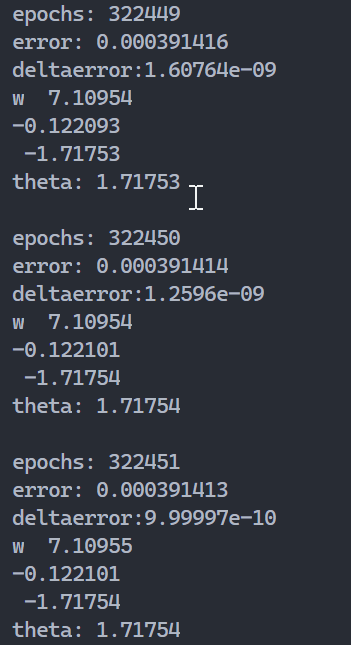
\includegraphics[width=0.2\textwidth]{image/online}
	\caption{Online Learning Method (batchsize = 1)}
\end{figure}

% \begin{figure}[H]
% 	\centering
% 	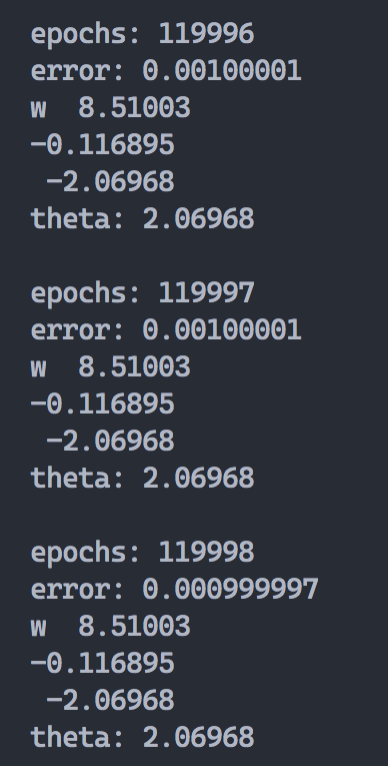
\includegraphics{image/100batch}
% 	\caption{Batch Method (batchsize = 100)}
% \end{figure}

\begin{figure}[h]
	\centering
	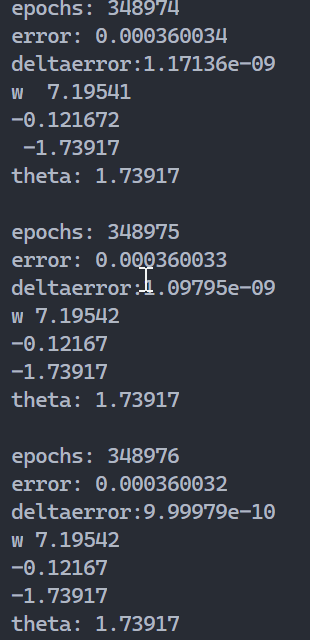
\includegraphics[width=0.2\textwidth]{image/3batch}
	\caption{Batch Method (batchsize = 3)}
\end{figure}

\end{homeworkProblem}

\end{document}
